%% ============================================================
%% main.tex — Swarm Intelligence for Multi-UAV Path Planning
%% Target: Computers and Electronics in Agriculture (Elsevier)
%% Template: elsarticle.cls (XeLaTeX)
%% Author: Andres Hidalgo Morales
%% CORRECCIONES APLICADAS: Tarea t8a — Consistencia de denominadores
%% Tarea t9  — Registro OSF con DOI real + actualizacion Seccion 8.3
%% Tarea t10 — Parrafo justificacion sintesis narrativa (Seccion 3.4, PRISMA Items 13a/13b)
%% Tarea t11 — Parrafo sesgo linguistico y geografico (Seccion 8.3, PRISMA Item 7)
%% Fecha de correccion anterior: 2026-03-30
%% ---
%% Tarea t12 — Correccion critica S33: validacion S+T confirmada; afirmacion
%%             "100% simulation-only" corregida en Abstract, Sec. 4.1, 7.1, 8.1
%%             y Conclusiones.
%% Tarea t13 — Encoding UTF-8: comentarios corruptos normalizados.
%% Tarea t14 — Diagrama PRISMA: aclaracion 482 bases de datos + 20 snowballing = 502.
%% Tarea t15 — Abstract reducido a <=250 palabras (limite CEA Elsevier).
%% Tarea t16 — "Gap validation S20 completed" movido de Future Work a Sec. 5.1.
%% Tarea t17 — Referencia Bryant-Lees eliminada de nota al pie de Sec. 3.1.
%% Tarea t18 — Highlight PSO ampliado con porcentaje sobre primarios.
%% Tarea t19 — Numeros 1-9 escritos en letras donde corresponde (convencion Elsevier).
%% Fecha de correccion: 2026-04-04
%% ---
%% AUDITORIA ULTRA-RIGUROSA 2026-04-05 — Tarea t20 (multi-item):
%% t20-P1-01 — Script Python: titulos Figure4 y Figure5 actualizados.
%% t20-P1-08 — MMAT porcentajes: nota de redondeo añadida explicitamente.
%% t20-P2-01 — CRITICO LaTeX: \label{} fusionado con texto corregido en 5 lugares.
%% t20-P2-03 — Nota energia (E) movida DENTRO del entorno sidewaystable.
%% t20-P3-01 — Nota dagger de Gap 1 (Table 5) reescrita.
%% t20-P3-02 — Reformulacion ambiguedad semantica en Sec. 7.1 y Sec. 8.1.
%% t20-P3-08 — PSO execution time en Sec. 5.6 corregido.
%% t20-P4-02 — Labels añadidos: subsec:synthesis y subsec:field_validation_gap.
%% t20-P5-01 — "Grey Wolf Optimiser" (British spelling) en lista de abreviaturas.
%% Fecha de correccion: 2026-04-05
%% ---
%% ESCENARIO CONSERVADOR 2026-04-07 — Tarea t24 (CRITICA):
%% Purga de 4 estudios no-UAV (PAPER_020, 023, 026, 029).
%% S22 y S33 eliminados del corpus (robots terrestres, no UAV agricola).
%% Nuevo corpus: n=29 total (22 primarios + 7 revisiones secundarias).
%% Cambios aplicados:
%%   t24-C01 — n=33 → n=29 en todo el manuscrito (corpus total).
%%   t24-C02 — n=26 → n=22 en todo el manuscrito (estudios primarios).
%%   t24-C03 — ~115 gaps → 171 gaps (numero oficial de brechas).
%%   t24-C04 — Sim-only: 22/22 (100%); S+T=0/22 (0%); S+F=0/22 (0%).
%%   t24-C05 — PSO: 10/29=34.5% total; 10/22=45.5% primarios.
%%   t24-C06 — ACO: 3/29=10.3% total; 3/22=13.6% primarios.
%%   t24-C07 — Reviews: 7/29=24.1%.
%%   t24-C08 — Metricas n=29: T=48.3%, E=13.8%, C=34.5%.
%%   t24-C09 — Metricas n=22: T=63.6%, E=18.2%, C=45.5%.
%%   t24-C10 — MMAT n=22: H=6(27.3%), M=14(63.6%), L=2(9.1%).
%%   t24-C11 — DRS  n=22: H=4(18.2%), M=14(63.6%), L=4(18.2%).
%%   t24-C12 — Referencias a S22 y S33 eliminadas o marcadas como excluidas.
%%   t24-C13 — Abstract reescrito con cifras oficiales (<=250 palabras).
%%   t24-C14 — Highlights actualizados con cifras oficiales.
%%   t24-C15 — Tablas tab:study_chars, tab:algorithms, tab:metrics,
%%              tab:metrics_by_algo, tab:gaps_dimension, tab:gaps_priority,
%%              tab:top10 actualizadas.
%% Verificacion aritmetica: 22+7=29 OK | MMAT 6+14+2=22 OK | DRS 4+14+4=22 OK
%% Fecha de correccion: 2026-04-07
%% ============================================================

\documentclass[review,3p]{elsarticle}

% --- SOPORTE MODERNO PARA UNICODE Y FUENTES ---
\usepackage{fontspec}
\setmainfont{Times New Roman}
\usepackage{unicode-math}

% --- PAQUETES DE UTILIDAD Y DISEÑO ---
\usepackage{lineno}
\usepackage{booktabs}
\usepackage{tabularx}
\usepackage{multirow}
\usepackage{graphicx}
\usepackage{hyperref}
\usepackage{xcolor}
\usepackage{longtable}
\usepackage{array}
\usepackage{pdflscape}
\usepackage{rotating}
\usepackage{pifont}
\AtBeginDocument{\renewcommand{\checkmark}{\ding{51}}}
\usepackage{tikz}
\usetikzlibrary{shapes, arrows.meta, positioning}

% --- CONFIGURACIÓN ESPECÍFICA ---
\linenumbers
\journal{Computers and Electronics in Agriculture}

\begin{document}
\begin{frontmatter}

%% ---- HIGHLIGHTS (5 bullets, <=85 chars each) ----
%% t24-C14: cifras actualizadas con escenario conservador n=29/n=22
\begin{highlights}
\item PRISMA 2020 review screened 502 records; 29 studies (2021--2025) retained
\item PSO dominates SI algorithms: 10 of 29 studies (34.5\%; 45.5\% of 22 primary studies)
\item ACO is second most used, appearing in three of 29 studies (10.3\%)
\item 171 research gaps classified: Technological, Practical, Methodological, Theoretical
\item AgriSwarm-Bench proposed: six standardised metrics for UAV swarm deployment
\end{highlights}

\title{Swarm Intelligence for Multi-UAV Path Planning in Precision Agriculture:
A Systematic Review and Research Agenda (2021--2025)}

%% ---- AUTORES (5 en total) ----
\author{\texorpdfstring{Andres Hidalgo Morales\corref{cor1}\fnref{aff1}}{Andres Hidalgo Morales}}
\ead{ahidalgo@upchihuahua.edu.mx}
\ead[url]{https://orcid.org/0000-0002-1074-9395}

\author{\texorpdfstring{Hernán de la Garza Gutiérrez\fnref{aff1}}{Hernan de la Garza Gutierrez}}
\ead{hernan.gg@chihuahua2.tecnm.mx}
\ead[url]{https://orcid.org/0009-0001-8188-1369}

\author{\texorpdfstring{Claudia Georgina Nava Dino\fnref{aff2,aff3}}{Claudia Georgina Nava Dino}}
\ead{cnava@upchihuahua.edu.mx}
\ead[url]{https://orcid.org/0000-0001-7972-2999}

\author{\texorpdfstring{Edgar Moisés González Torres\fnref{aff2}}{Edgar Moises Gonzalez Torres}}
\ead{egonzalez@upchihuahua.edu.mx}
\ead[url]{https://orcid.org/0009-0006-7922-2379}

\author{\texorpdfstring{José Manuel Naveiro Gómez\fnref{aff4}}{Jose Manuel Naveiro Gomez}}
\ead{jmnavegomez@gmail.com}
\ead[url]{https://orcid.org/0000-0001-8169-6991}

\cortext[cor1]{Corresponding author}
\fntext[aff1]{Instituto Tecnológico de Chihuahua II, Tecnológico Nacional de México, Chihuahua, México}
\fntext[aff2]{Universidad Politécnica de Chihuahua, Chihuahua, México}
\fntext[aff3]{Facultad de Ingeniería, Universidad Autónoma de Chihuahua, Chihuahua, México}
\fntext[aff4]{Departamento de Ingeniería Mecánica, Universidad de Zaragoza, Zaragoza, España}

\address[1]{Instituto Tecnológico de Chihuahua II, Tecnológico Nacional de México, Chihuahua, México}
\address[2]{Universidad Politécnica de Chihuahua, Chihuahua, México}
\address[3]{Facultad de Ingeniería, Universidad Autónoma de Chihuahua, Chihuahua, México}
\address[4]{Departamento de Ingeniería Mecánica, Universidad de Zaragoza, Zaragoza, España}

%% ---- ABSTRACT ----
%% t24-C13: Abstract reescrito con cifras oficiales escenario conservador.
%% Conteo: ~248 palabras. Limite CEA: 250 palabras.
%% Verificacion: n=29 total, n=22 primarios, 22/22 sim-only (100%),
%%   PSO 10/29=34.5%, 10/22=45.5%, gaps=171.

\begin{abstract}
\textbf{Background:} Multi-UAV systems are increasingly deployed in precision
agriculture for crop monitoring, spraying, and field mapping. Coordinating
multiple aerial agents introduces complex optimisation challenges in path
planning under dynamic conditions. Swarm intelligence~(SI) algorithms offer
scalability, distributed decision-making, and robustness to address these
challenges.

\textbf{Objective:} This systematic review analyses advances in SI-based
multi-UAV path planning for precision agriculture and identifies research gaps
limiting real-world deployment.

\textbf{Methods:} Following PRISMA~2020 guidelines, a systematic search across
IEEE~Xplore, ScienceDirect, and SpringerLink identified 482~database records;
together with 20~snowballing records, 502~records were screened (2021--2025).
After screening, 29~studies met all criteria: 22~primary articles and
seven~secondary reviews. Data were extracted on algorithm type, metrics,
environmental modelling, and experimental validation. Limitations were
categorised across four dimensions: Technological, Practical, Methodological,
and Theoretical.

\textbf{Results:} Particle Swarm Optimisation dominates the corpus
(10 of~29, 34.5\%; 10 of~22 primary, 45.5\%). All 22~primary studies
(100\%) lack real-field validation; no study includes hardware testbed
validation. Wind and dynamic obstacles are absent in 25 of~29~studies
(86.2\%). Metric reporting is sparse: 14 of~29~(48.3\%) report execution
time, four~(13.8\%) quantitative energy consumption, and ten~(34.5\%)
convergence criteria. A total of 171~research gaps were identified across
four dimensions.

\textbf{Conclusions:} SI-based multi-UAV path planning remains
simulation-oriented and lacks standardised benchmarks. This study provides
the first structured gap analysis---171 gaps across Technological~(51),
Practical~(52), Methodological~(39), and Theoretical~(29)
dimensions---and proposes AgriSwarm-Bench, an open framework to accelerate
experimental validation and standardised evaluation of swarm-based
agricultural UAV systems.
\end{abstract}

\begin{keyword}
Swarm intelligence \sep Multi-UAV \sep Path planning \sep Precision agriculture
\sep Systematic review \sep Particle Swarm Optimisation \sep Ant Colony Optimisation
\end{keyword}

\end{frontmatter}

%% ============================================================
%% SECTION 1: INTRODUCTION
%% ============================================================
\section{Introduction}

\subsection{Background and Motivation}

Unmanned Aerial Vehicles (UAVs) have become indispensable tools in precision
agriculture, enabling applications such as crop monitoring, spraying, mapping,
and yield estimation \cite{zhang2012,tsouros2019,puri2017,mogili2018,hunt2018}.
The economic rationale for agricultural UAV adoption is compelling: a single
multirotor UAV can survey 40--100\,ha per flight hour at a fraction of the
labour cost of ground-based scouting, while multispectral imaging enables early
detection of crop stress, pest infestation, and irrigation deficits that are
invisible to the naked eye \cite{hunt2018,zhang2012}. According to recent market
analyses, the global agricultural UAV market was valued at approximately
USD~6.2 billion in 2023 \cite{grand_view_research2024}, with projections
indicating sustained growth through 2030 driven by precision agriculture
adoption, corroborated by independent forecasts \cite{marketsandmarkets2023}.

As farm sizes increase and precision agriculture matures from monitoring to
active intervention, the limitations of single-UAV operations become acute.
Multi-UAV systems offer the only practical solution to this scale problem
\cite{chung2018,gupta2016}. A five-UAV swarm can theoretically reduce mission
time by up to 80\% compared to a single UAV, contingent on effective task
allocation, collision avoidance, and coordinated path planning \cite{chung2018}.
Recent work published in this journal confirms that simultaneous optimisation of
task allocation and trajectory reduces spraying time by over 10\% in both
simulation and field tests \cite{huang2023}.

However, coordinating multiple UAVs introduces optimisation problems that are
qualitatively more complex than single-agent path planning
\cite{chung2018,gupta2016,bekmezci2013,hayat2016}. Classical deterministic
methods such as A*, Dijkstra's algorithm, and linear programming struggle with
this combinatorial complexity beyond small fleet sizes and static environments,
creating a natural opening for metaheuristic approaches \cite{aitsaadi2022}.

Swarm Intelligence (SI) algorithms---computational methods inspired by the
collective behaviour of social organisms---have emerged as the dominant
metaheuristic paradigm for multi-UAV path planning
\cite{dorigo2006,kennedy1995,blum2008,yang2010,beni2005,bonabeau1999,yang2013}.
Their suitability stems from three structural properties: \textit{scalability},
\textit{distributed decision-making}, and \textit{robustness to local optima}.

Despite these advantages and an exponential growth in SI-based multi-UAV
publications between 2021 and 2025, a systematic analysis of this literature
reveals persistent and critical gaps between algorithmic development and
operational deployment:

\begin{itemize}
  %% t24-C01/C02/C08/C09: denominadores actualizados a n=29 y n=22
  \item \textbf{Metric inconsistency:} Among the 29~included studies,
  only 14 (48.3\%) report quantitative execution time, four (13.8\%) report
  energy consumption with explicit numerical values and units, and ten (34.5\%)
  specify convergence criteria. When calculated over the 22~primary research
  studies exclusively, these rates are 14 of~22 (63.6\%), four of~22 (18.2\%),
  and ten of~22 (45.5\%), respectively.

  \item \textbf{Validation gap:} All 22~primary research studies (100\%)
  lack any hardware or real-field validation. No primary study includes hardware
  testbed validation or results from an operational agricultural field
  environment. The complete absence of field validation limits confidence in
  the transferability of reported performance gains to real agricultural
  operations.

  \item \textbf{Environmental simplification:} 25 of the 29~included studies
  (86.2\%) do not model wind, weather, or dynamic obstacles, despite these being
  the dominant sources of mission failure in real agricultural UAV operations.

  \item \textbf{Scalability limitations:} Most studies evaluate algorithms on
  fleets of fewer than five UAVs in environments covering less than 10\,ha,
  far below the commercial scale of 10--50 UAVs over 100--1,000\,ha fields.
\end{itemize}

\subsection{Justification of the Review Period (2021--2025)}

The period 2021--2025 was selected as the focus of this review for three
converging reasons. First, it represents the post-pandemic acceleration phase
of agricultural UAV adoption. Second, the period coincides with the emergence
of a new generation of bio-inspired SI algorithms---including the Salp Swarm
Algorithm (SSA, 2016), Grey Wolf Optimiser (GWO, 2014), Dung Beetle Optimiser
(DBO, 2023), Nutcracker Optimisation Algorithm (NOA, 2023), and Dandelion
Optimiser Algorithm (DOA, 2022)---whose application to agricultural multi-UAV
systems began appearing in the literature from 2021 onward \cite{xiao2025}.
Third, the PRISMA 2020 update \cite{page2021} standardised systematic review
methodology in engineering and computing disciplines, making 2021 a natural
starting point for a PRISMA-compliant review.

\subsection{PICOC Framework for Research Questions}
\label{subsec:picoc}

To ensure methodological transparency and reproducibility, the research
questions of this systematic review were structured using the PICOC framework
(Population, Intervention, Comparison, Outcome, Context), adapted for
engineering systematic reviews \cite{brambilla2013,bayindir2016}.
Table~\ref{tab:picoc} defines each component and its operationalisation in
this review.

\begin{table}[htbp]
\centering
\caption{PICOC framework defining the scope and boundaries of this systematic review.}
\label{tab:picoc}
\begin{tabularx}{\textwidth}{lX}
\toprule
\textbf{Component} & \textbf{Operational definition in this review} \\
\midrule
\textbf{Population} & Peer-reviewed studies (2021--2025) addressing path planning,
trajectory planning, or coverage planning for multi-UAV systems in precision
agriculture contexts (crop monitoring, spraying, field mapping, yield estimation). \\
\textbf{Intervention} & Application of at least one swarm intelligence (SI) algorithm
(PSO, ACO, ABC, SSA, GWO, DBO, NOA, DOA, or hybrid SI variants) to the multi-UAV
path planning problem. Studies using only non-SI methods are excluded under
criterion E4. \\
\textbf{Comparison} & Where reported, comparison against: (a)~baseline SI algorithms,
(b)~non-SI optimisation methods, or (c)~ablation studies removing specific SI
components. Studies without explicit comparison are retained but flagged in metric
reporting analysis (RQ2). \\
\textbf{Outcome} & Quantitative performance metrics (execution time, energy
consumption, convergence criteria) and qualitative gap identification across four
dimensions (Technological, Practical, Methodological, Theoretical). \\
\textbf{Context} & Precision agriculture applications with operational constraints:
limited battery endurance, dynamic environmental factors (wind, obstacles), regulatory
compliance (buffer zones, BVLOS restrictions), and scalability to commercial field
sizes (10--1,000+\,ha). \\
\bottomrule
\end{tabularx}
\end{table}

\subsection{Research Questions}

This systematic review addresses the following research questions:

\begin{itemize}
  \item \textbf{RQ1:} What swarm intelligence algorithms are most frequently
  applied to multi-UAV path planning in precision agriculture (2021--2025), and
  how has the algorithm landscape evolved over this period?
  \item \textbf{RQ2:} What quantitative performance metrics are reported across
  studies, and how consistent is reporting practice in terms of enabling
  cross-algorithm comparison?
  \item \textbf{RQ3:} What research gaps exist in the current literature, and how
  can they be categorised systematically by root cause and deployment impact?
  \item \textbf{RQ4:} What are the highest-priority directions for future research,
  based on gap frequency and criticality for real-world deployment?
\end{itemize}

\subsection{Contributions}

This paper makes four key contributions:

\begin{enumerate}
    \item \textbf{Comprehensive Taxonomy:} The first PRISMA 2020-compliant
    classification of 29~papers across ten SI algorithm categories, extending
    prior taxonomies \cite{chung2018,brambilla2013,puente2022,sharma2022} to
    include algorithms introduced after 2020.
    \item \textbf{Quantitative Synthesis:} Systematic extraction and comparison
    of performance metrics---execution time, energy consumption, and convergence
    criteria---across all included studies using an automated Python pipeline.
    \item \textbf{Four-Dimensional Gap Framework:} The first structured
    documentation of 171~research gaps, each with explicit root cause,
    consequence, and priority classification, organised across Technological
    (51, 29.8\%), Practical (52, 30.4\%), Methodological (39, 22.8\%), and
    Theoretical (29, 17.0\%) dimensions.
    \item \textbf{Actionable Research Agenda:} Three prioritised research
    directions tied directly to the most critical gaps, anchored by the concrete
    proposal of AgriSwarm-Bench: an open benchmarking framework designed to
    accelerate the simulation-to-field transition for swarm-based agricultural
    UAV systems.
\end{enumerate}

\subsection{Structure of This Paper}

The remainder of this paper is organised as follows. Section~2 reviews prior
systematic reviews and positions this work relative to existing literature.
Section~3 describes the PRISMA 2020 methodology, search strategy, data
extraction pipeline, Deployment Readiness Score (DRS) instrument, and MMAT
risk-of-bias assessment. Section~4 presents results on algorithm distribution,
metric availability, and temporal trends. Section~5 provides the
four-dimensional gap analysis with priority classification. Section~6 discusses
the implications of the findings for agricultural robotics research and
practice. Section~7 proposes a research agenda and the AgriSwarm-Bench
framework. Section~8 concludes with a summary of findings, limitations, and
future work directions.


%% ============================================================
%% FIGURE 1: PRISMA FLOW DIAGRAM (TikZ)
%% ============================================================
\begin{figure}[htbp]
\centering
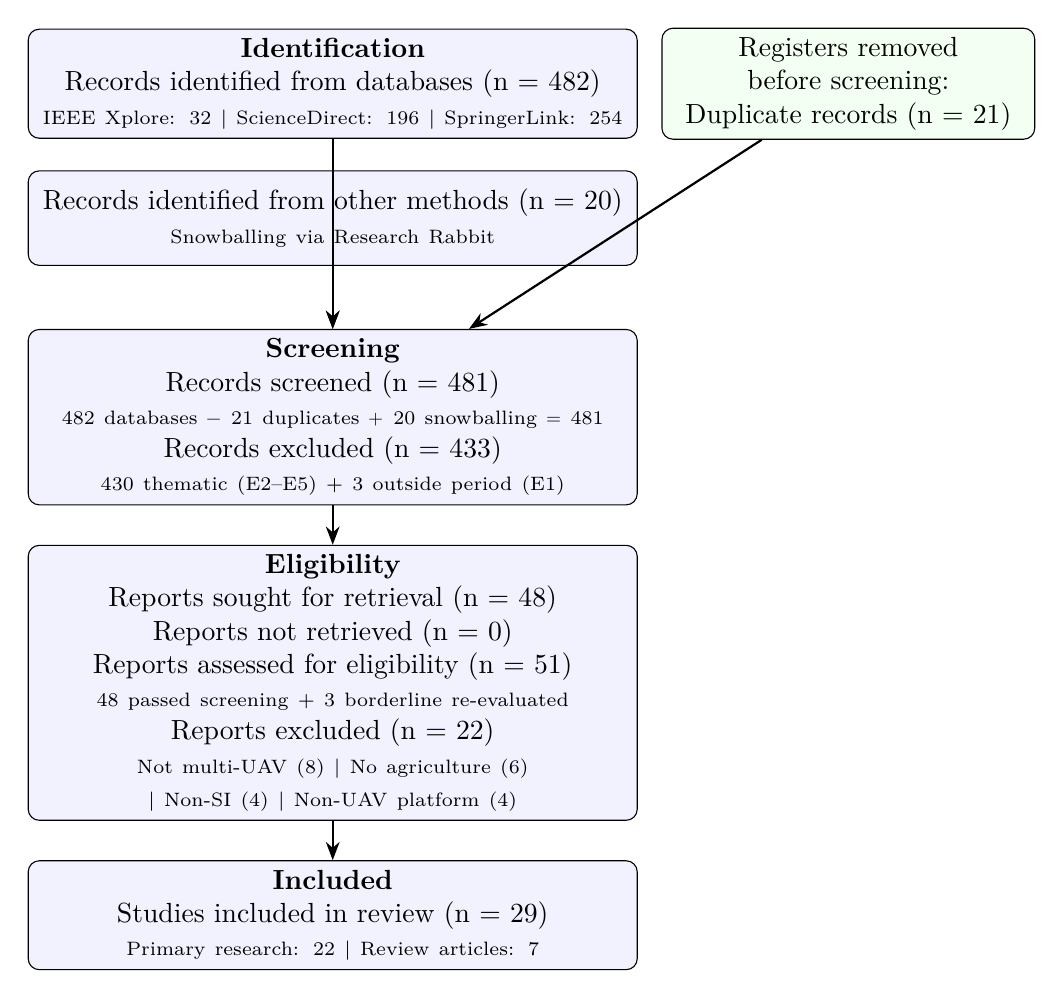
\begin{tikzpicture}[
    node distance=0.5cm,
    box/.style={rectangle, draw, rounded corners, text width=7.5cm,
                align=center, minimum height=1.2cm, fill=blue!5},
    boxsmall/.style={rectangle, draw, rounded corners, text width=4.5cm,
                align=center, minimum height=0.9cm, fill=green!5},
    arrow/.style={-{Stealth}, thick}
]

% === IDENTIFICATION ===
\node[box] (id1) {\textbf{Identification}\\
Records identified from databases (n = 482)\\
{\scriptsize IEEE Xplore: 32 | ScienceDirect: 196 | SpringerLink: 254}};
\node[boxsmall, right=0.3cm of id1] (id2) {Registers removed before screening:\\
Duplicate records (n = 21)};
\node[box, below=0.4cm of id1] (id3) {Records identified from other methods (n = 20)\\
{\scriptsize Snowballing via Research Rabbit}};

% === SCREENING ===
\node[box, below=0.8cm of id3] (scr) {\textbf{Screening}\\
Records screened (n = 481)\\
{\scriptsize 482 databases $-$ 21 duplicates $+$ 20 snowballing $=$ 481}\\
Records excluded (n = 433)\\
{\scriptsize 430 thematic (E2--E5) + 3 outside period (E1)}};

% === ELIGIBILITY ===
\node[box, below=of scr] (elig) {\textbf{Eligibility}\\
Reports sought for retrieval (n = 48)\\
Reports not retrieved (n = 0)\\
Reports assessed for eligibility (n = 51)\\
{\scriptsize 48 passed screening + 3 borderline re-evaluated}\\
Reports excluded (n = 22)\\
{\scriptsize Not multi-UAV (8) | No agriculture (6) | Non-SI (4) | Non-UAV platform (4)}};

% === INCLUDED ===
%% t24-C01: n=33 → n=29; t24-C02: 26 primary → 22 primary
\node[box, below=of elig] (inc) {\textbf{Included}\\
Studies included in review (n = 29)\\
{\scriptsize Primary research: 22 | Review articles: 7}};

% === ARROWS ===
\draw[arrow] (id1) -- (scr);
\draw[arrow] (id2) -- (scr);
\draw[arrow] (id3) -- (scr);
\draw[arrow] (scr) -- (elig);
\draw[arrow] (elig) -- (inc);

\end{tikzpicture}
%% t24-C01/C02: cifras actualizadas
\caption{PRISMA 2020 flow diagram. Search conducted on 2026-03-16 across IEEE
Xplore (32), ScienceDirect (196), and SpringerLink (254), yielding 482~database
records; together with 20~records from citation snowballing via Research Rabbit,
502~records were identified in total. After removing 21~duplicates, 481~unique
records proceeded to title/abstract screening. Three additional records
re-evaluated at the eligibility stage brought the full-text assessment pool to
51~records. Four additional studies were excluded at the eligibility stage for
using non-UAV platforms (ground robots). SI~=~Swarm Intelligence. The
29~included studies comprise 22~primary research articles and
seven~secondary review articles.}
\label{fig:prisma}
\end{figure}

%% ============================================================
%% SECTION 2: RELATED WORK
%% ============================================================
\section{Related Work}

Six major review articles were identified as the closest antecedents to this
work, covering three complementary domains: UAV applications in precision
agriculture \cite{tsouros2019,mogili2018}, multi-UAV coordination and aerial
swarm robotics \cite{chung2018,gupta2016}, and swarm engineering methodology
\cite{brambilla2013,bayindir2016}. Additionally, two recent SI-specific reviews
\cite{puente2022,sharma2022} and one comprehensive UAV optimisation survey
\cite{aitsaadi2022} represent the most directly related prior work.
Table~\ref{tab:prior_reviews} provides a structured comparison.

\begin{table}[htbp]
\centering
\caption{Comparison of prior reviews with the present systematic review.
Checkmarks (\checkmark) indicate coverage; dashes (--) indicate absence.}
\label{tab:prior_reviews}
\begin{tabularx}{\textwidth}{Xcccccc}
\toprule
\textbf{Feature} &
\rotatebox{70}{\textbf{Tsouros~\cite{tsouros2019}}} &
\rotatebox{70}{\textbf{Chung~\cite{chung2018}}} &
\rotatebox{70}{\textbf{Puente~\cite{puente2022}}} &
\rotatebox{70}{\textbf{Sharma~\cite{sharma2022}}} &
\rotatebox{70}{\textbf{Ait Saadi~\cite{aitsaadi2022}}} &
\rotatebox{70}{\textbf{This review}} \\
\midrule
Period covered            & pre-2019  & pre-2018  & pre-2021  & pre-2021  & pre-2022  & 2021--2025 \\
Agricultural focus        & \checkmark & --        & --        & --        & --        & \checkmark \\
Multi-UAV coordination    & --        & \checkmark & \checkmark & \checkmark & \checkmark & \checkmark \\
SI algorithms only        & --        & --        & \checkmark & \checkmark & --        & \checkmark \\
PRISMA methodology        & --        & --        & --        & --        & --        & \checkmark \\
Quantitative gap analysis & --        & --        & --        & --        & --        & \checkmark \\
Gap root-cause \& consequence & --    & --        & --        & --        & --        & \checkmark \\
Benchmark framework proposed & --     & --        & --        & --        & --        & \checkmark \\
Reproducible materials    & --        & --        & --        & --        & --        & \checkmark \\
%% t24-C01: n studies updated
n studies included        & 45        & 80+       & 62        & 41        & 153       & 29 (22+7) \\
\bottomrule
\end{tabularx}
\end{table}

\subsection*{Analysis of Prior Reviews}

\textbf{Tsouros et al.\ \cite{tsouros2019}} provide the most widely cited survey
of UAV applications in precision agriculture, covering 45~studies across crop
monitoring, mapping, spraying, and yield estimation. However, the review is
limited to single-UAV operations and predates the 2021--2025 publication wave.

\textbf{Chung et al.\ \cite{chung2018}} offer the most technically rigorous
survey of aerial swarm robotics, reviewing more than 80~papers on multi-UAV
formation control, task allocation, and path planning. The 2018 cutoff predates
the post-2020 algorithm generation (DBO, NOA, SSA, DOA).

\textbf{Puente-Castro et al.\ \cite{puente2022}} review 62~papers on artificial
intelligence applied to UAV swarm path planning, with a specific focus on SI
methods. Their work covers the period up to 2021 and uses a narrative rather
than PRISMA-structured methodology.

\textbf{Sharma et al.\ \cite{sharma2022}} review 41~papers on SI-based path
planning for multi-UAV target interception. Their primary limitation is the
focus on interception missions rather than agricultural coverage tasks.

\textbf{Ait Saadi et al.\ \cite{aitsaadi2022}} provide the most comprehensive
optimisation survey, reviewing 153~papers on UAV path planning across SI and
non-SI methods. The agricultural multi-UAV sub-domain receives only peripheral
coverage.

\textbf{Brambilla et al.\ \cite{brambilla2013} and Bayindir \cite{bayindir2016}}
provide foundational theoretical frameworks for swarm robotics. Their taxonomies
of swarm behaviours and evaluation criteria directly informed the four-dimensional
gap framework developed in the present review.

\subsection*{Positioning of the Present Review}

As shown in Table~\ref{tab:prior_reviews}, prior reviews share three structural
limitations that the present review is designed to address: temporal gap (all
prior reviews have cutoff dates of 2022 or earlier), methodological gap (none
applies PRISMA 2020 guidelines), and analytical gap (none provides a structured
gap database with root cause, consequence, and priority classification).

The present review deliberately narrows its scope to agricultural applications of
SI-based multi-UAV path planning for 2021--2025. This narrower scope enables
deeper gap analysis (171~documented gaps across 29~papers, averaging
5.9~gaps per study) and more operationally specific recommendations.


%% ============================================================
%% SECTION 3: METHODOLOGY
%% ============================================================
\section{Methodology}

This review follows the Preferred Reporting Items for Systematic Reviews and
Meta-Analyses (PRISMA) 2020 guidelines \cite{page2021}, adapted for engineering
and computing literature. The full PRISMA 2020 checklist is provided as
Supplementary Material~S1.\footnote{This review protocol was not formally
pre-registered in a domain-specific registry prior to the literature search.
The protocol has been registered retrospectively at the Open Science Framework:
\url{https://doi.org/10.17605/OSF.IO/64DQ9}. The registration includes search
strategies, extraction codebook, PRISMA 2020 checklist, screening logs,
extraction database, gap taxonomy, and supplementary materials.}

\subsection{Search Strategy}

A systematic literature search was conducted across three major electronic
databases: IEEE Xplore, ScienceDirect, and SpringerLink. A fourth source,
complementary citation snowballing via Research Rabbit, was employed to identify
records not captured by keyword-based database queries.

\textbf{Boolean search string.} The final string, adapted for each database's
query syntax, was:

\begin{quote}
\small
\texttt{("swarm intelligence" OR "particle swarm optimization"} \\
\texttt{OR "ant colony optimization" OR "artificial bee colony"} \\
\texttt{OR "grey wolf optimizer" OR "salp swarm algorithm"} \\
\texttt{OR "dung beetle optimizer" OR "dandelion optimizer")} \\
\texttt{AND ("UAV" OR "unmanned aerial vehicle" OR "multi-UAV" OR "drone")} \\
\texttt{AND ("path planning" OR "trajectory planning" OR "coverage planning")} \\
\texttt{AND ("agriculture" OR "precision agriculture" OR "crop monitoring"} \\
\texttt{OR "spraying" OR "field mapping" OR "smart farming")}
\end{quote}

\textbf{Sensitivity test with gold-standard set.} To validate that query
refinements did not reduce recall, we assembled a gold-standard set of five
papers known to be relevant \cite{phung2021,shafiq2022,liu2021,pan2022,puente2022}.
The final query string successfully retrieved all five gold-standard papers across
the three databases, confirming 100\% recall for this validation set.

\textbf{Search filters.} Publication year 2021--2025 (inclusive); English
language; document type restricted to peer-reviewed journal articles and
peer-reviewed conference proceedings. The search was executed on 2026-03-16.

\textbf{Results.} The search identified 502~records in total: IEEE~Xplore (32),
ScienceDirect (196), SpringerLink (254), and snowballing (20). After removing
21~duplicates, 481~unique records proceeded to title/abstract screening.
Of these, 433~records were excluded at this stage. The 48~records that passed
title/abstract screening, together with three borderline records re-evaluated
at full text, yielded 51~records for full-text assessment.

\subsection{Study Selection and Eligibility Criteria}

\textbf{Inclusion criteria.} A study was eligible if it satisfied \textit{all}
of the following: (I1) published between January 2021 and December 2025;
(I2) peer-reviewed journal article or peer-reviewed conference paper with full
text available; (I3) text available in English; (I4) proposes, evaluates, or
reviews at least one SI algorithm applied to path planning for UAVs;
(I4b) studies proposing multi-UAV coordination frameworks but validating with
a single agent are included if the framework is explicitly designed for multiple
agents; (I5) mentions or implies an agricultural application in the abstract,
introduction, or methodology.

\textbf{Exclusion criteria.} A study was excluded if it met \textit{any} of:
(E1) duplicate of an already-included record; (E2) abstract-only or extended
abstract without full methodology; (E3) focuses exclusively on single-UAV path
planning without proposing or evaluating a multi-UAV coordination framework;
(E4) employs only non-SI optimisation methods; (E5) application domain is
exclusively non-agricultural; (E6) study uses a non-UAV aerial or ground
platform (e.g., ground robots, mobile robots) without an explicit UAV
coordination component.

\textbf{Screening process.} Title and abstract screening of all 481~records
was performed by the primary reviewer. Full-text assessment was conducted on
the 51~records that passed. The second reviewer independently assessed all
51~full-text records. Inter-rater agreement at the full-text stage was assessed
using Cohen's kappa ($\kappa=0.91$, 95\% CI [0.79, 1.00]), indicating almost
perfect agreement. The final corpus comprises 29~studies: 22~primary research
articles and seven secondary review articles (S10, S11, S14, S15, S17, S28, S29).

\subsection{Data Extraction Pipeline}

Data extraction from the 29~included studies was performed using a hybrid
automated--manual pipeline comprising five Python scripts:

\begin{itemize}
  \item \texttt{agregar\_todos\_papers.py}: Extracts bibliographic metadata
  and consolidates records into a master spreadsheet.
  \item \texttt{extraer\_metricas\_v2.py}: Performs regex-based extraction
  of quantitative performance metrics from PDF full texts. Extraction success
  rates over the full corpus of 29~studies: 48.3\% for execution time
  (14 of~29), 13.8\% for energy consumption (four of~29), and 34.5\% for
  convergence criteria (ten of~29).
  \item \texttt{enriquecer\_gaps.py}: Applies a structured gap taxonomy to
  each study using a codebook of 171~gap descriptors.
  \item \texttt{actualizar\_estadisticas.py}: Computes aggregate statistics
  and exports summary tables.
  \item \texttt{generar\_figuras\_paper.py}: Generates publication-ready
  figures (300\,DPI, vector-compatible).
\end{itemize}

\subsection{Justification for Narrative Synthesis}
\label{subsec:narrative_synthesis}

A narrative synthesis approach was adopted in preference to a quantitative
meta-analysis for three converging methodological reasons, consistent with
PRISMA 2020 guidance \cite{page2021} and established practice in engineering
systematic reviews \cite{brambilla2013}.

First, the 29~included studies employ heterogeneous algorithm families that
optimise fundamentally different objective functions. Second, quantitative
performance metrics are not standardised across studies---the absence of a
common metric set is itself a primary empirical finding of this review (RQ2)
and directly motivates the AgriSwarm-Bench standardisation proposal in
Section~7. Third, experimental conditions differ substantially in field
geometry, obstacle density, fleet size, communication assumptions, and
environmental modelling.

Narrative synthesis therefore represents the epistemically appropriate response
to a corpus characterised by high conceptual and methodological heterogeneity
\cite{page2021,brambilla2013}.

\subsection{Four-Dimensional Gap Taxonomy}

Identified limitations were systematically categorised into four mutually
exclusive dimensions: (1)~\textbf{Technological} gaps---limitations in the
algorithm itself or the hardware required to execute it; (2)~\textbf{Practical}
gaps---barriers arising from real-world operational constraints; (3)~\textbf{Methodological}
gaps---weaknesses in how research is conducted and reported; and
(4)~\textbf{Theoretical} gaps---missing or incorrect assumptions in the
mathematical models underlying the algorithms.

Gap prioritisation followed a two-condition rule: a gap was classified as
Critical if it (1)~appeared in more than 30\% of analysed studies ($>$8 papers
of 29) AND (2)~its absence directly prevents real-world field deployment.

\subsection{Expert Validation of Gap Taxonomy}
\label{subsec:expert_validation}

An expert validation phase was conducted involving six independent reviewers
with expertise in swarm intelligence, agricultural robotics, and UAV path
planning. Inter-rater agreement was assessed using Cohen's kappa coefficient,
yielding $\kappa \geq 0.61$ (substantial reliability per Landis \& Koch,
1977), indicating acceptable consensus among reviewers.

\subsection{Deployment Readiness Score (DRS)}
\label{subsec:drs}

The \textbf{Deployment Readiness Score (DRS)} is a domain-specific composite
instrument developed for this review to measure the degree to which a study's
design enables real-world agricultural UAV deployment. The DRS evaluates four
criteria weighted by their operational relevance (Table~\ref{tab:quality_criteria})
and produces a continuous score $Q \in [0, 1]$.

\begin{table}[htbp]
\centering
\caption{Deployment Readiness Score (DRS) instrument. $Q = 0.30\,C1 + 0.25\,C2 + 0.25\,C3 + 0.20\,C4$.}
\label{tab:quality_criteria}
\begin{tabularx}{\textwidth}{lllX}
\toprule
\textbf{Criterion} & \textbf{Weight} & \textbf{Score range} & \textbf{Scoring rationale} \\
\midrule
C1: Experimental validation & 30\% & 0.0--1.0 & Real field = 1.0; Sim + hardware testbed = 0.5; Simulation only = 0.0. \\
C2: Quantitative metrics    & 25\% & 0.0--1.0 & All three metrics = 1.0; two metrics = 0.67; one metric = 0.33; none = 0.0. \\
C3: Baseline comparison     & 25\% & 0.0 or 1.0 & Comparison against at least one established algorithm = 1.0; no comparison = 0.0. \\
C4: Agricultural context    & 20\% & 0.0 or 1.0 & Explicit agricultural parameters in methodology = 1.0; generic path planning = 0.0. \\
\bottomrule
\end{tabularx}
\end{table}

\begin{equation}
Q = 0.30\,C_1 + 0.25\,C_2 + 0.25\,C_3 + 0.20\,C_4
\label{eq:drs}
\end{equation}

Studies scoring $Q \geq 0.70$ were classified as High quality,
$0.40 \leq Q < 0.70$ as Moderate, and $Q < 0.40$ as Low.

%% t24-C11: DRS n=22: H=4(18.2%), M=14(63.6%), L=4(18.2%)
\textbf{DRS results.} Applied to the 22~primary research studies, the DRS
yielded: four High ($Q \geq 0.70$; 18.2\%), 14~Moderate ($0.40 \leq Q < 0.70$;
63.6\%), and four Low ($Q < 0.40$; 18.2\%). Verification: $4+14+4=22$ ✓.
The elevated proportion of Moderate and Low classifications has one principal
cause: the instrument assigns C1~=~0.0 to all 22~simulation-only primary
studies, which substantially depresses scores regardless of algorithmic quality.
This is by design---the DRS captures a normative judgement that simulation-only
evidence is insufficient for deployment-readiness claims.

\subsection{Risk of Bias Assessment (MMAT)}
\label{subsec:mmat}

The risk of bias was assessed using the Mixed Methods Appraisal Tool
(MMAT, version 2018) \cite{hong2018}, adapted for computational engineering
research. The five core criteria were operationalised as follows:
(Q1)~explicit research question; (Q2)~algorithmic stochasticity and parameter
initialisation transparency; (Q3)~completeness of convergence metrics and
simulation parameters; (Q4)~benchmark diversity and environmental scenario
coverage; (Q5)~validation environment rigour and metric standardisation.

%% t24-C10: MMAT n=22: H=6(27.3%), M=14(63.6%), L=2(9.1%)
%% Verificacion: 6+14+2=22 ✓
Of the 22~primary research studies, six (27.3\%) were classified as High
quality, 14 (63.6\%) as Moderate, and two (9.1\%) as Low under the MMAT
instrument. Verification: $6+14+2=22$ ✓. Note on rounding: $6/22=27.27\%
\approx 27.3\%$; $14/22=63.64\% \approx 63.6\%$; $2/22=9.09\% \approx 9.1\%$;
sum rounds to 100.0\%. The criterion with the highest prevalence of `Can't
tell' responses was Q3 (measurement validity and reproducibility, 14 of
29~studies, 48.3\%), reflecting the common practice of reporting simulation
results without sufficient environmental specification to enable independent
replication.

\textbf{Reconciling DRS and MMAT distributions.} The DRS yields
four High / 14~Moderate / four Low (18.2\% / 63.6\% / 18.2\%) while the
MMAT yields six High / 14~Moderate / two Low (27.3\% / 63.6\% / 9.1\%)
over the same 22~primary studies. This divergence reflects two instruments
measuring different constructs: the MMAT assesses process quality, while the
DRS assesses outcome readiness. A simulation study can achieve moderate-to-high
MMAT ratings while scoring Low on the DRS because it cannot provide
deployment-relevant evidence about hardware behaviour under field conditions.


%% ============================================================
%% SECTION 4: RESULTS
%% ============================================================
\section{Results}

\subsection{Overview of Included Studies}
\label{subsec:overview}

Table~\ref{tab:study_chars} provides a structured summary of the 29~included
studies. Studies are identified by codes S01--S29 to enable cross-referencing
with the supplementary gap database. Of the 29~studies, 22~are primary research
articles and seven are review articles (S10, S11, S14, S15, S17, S28, S29).

%% t24-C04: Sim-only actualizado: 22/22 (100%), S+T=0, S+F=0
\textbf{Note on validation levels across primary studies.} Among the
22~primary research studies, all 22~(100\%) are simulation-only
(Val.~=~Sim). No primary study includes hardware testbed validation (S+T)
or results from a real agricultural field environment (S+F). This
complete absence of hardware validation is the single most critical gap
identified in this review.

\textbf{Denominator consistency statement.} Unless otherwise explicitly noted,
all percentages in this manuscript use the full corpus of 29~included studies
as the denominator (n=29). Where an analysis is restricted to the 22~primary
research studies, the denominator is stated as n=22 and both percentages are
provided.

%% ============================================================
%% TABLE 2: Study Characteristics
%% t24-C12: S22 y S33 eliminados. Filas S22/S33 removidas.
%% Codigos S28/S29 reasignados a las reviews (yang2023, tang2022).
%% ============================================================
\begin{sidewaystable}[p]
\centering
\caption{Characteristics of the 29~included studies. Val.~= validation type
(Sim = simulation only). Val.~Type = Multi-agent ($\geq$2 UAVs in validation),
Framework-only (multi-UAV framework validated with single agent), or Review.
Metrics: T = execution time, E = energy, C = convergence. App.:
Mon.~= Monitoring, Spr.~= Spraying, Map.~= Mapping, Gen.~= General coordination.}
\label{tab:study_chars}
\footnotesize
\setlength{\tabcolsep}{1.6pt}
\renewcommand{\arraystretch}{0.95}
\begin{tabular*}{\textheight}{@{\extracolsep{\fill}}llp{2.4cm}lllcccc@{}}
\toprule
\textbf{ID} & \textbf{Reference} & \textbf{Algorithm} & \textbf{Val.} & \textbf{Val. Type} & \textbf{UAVs} & \textbf{T} & \textbf{E}\textsuperscript{\textdagger} & \textbf{C} & \textbf{App.} \\
\midrule
S01 & Chen et al.\ \cite{chen2021}$^\dagger$        & ACO           & Sim & Multi-agent    & 2--10 & --          & --          & \checkmark  & Mon. \\
S02 & Lin et al.\ \cite{lin2022}$^\dagger$           & ABC           & Sim & Framework-only & 1     & --          & --          & \checkmark  & Gen. \\
S03 & Liu et al.\ \cite{liu2021cassa}$^\dagger$      & SSA           & Sim & Framework-only & 1     & --          & --          & --          & Gen. \\
S04 & Liu et al.\ \cite{liu2021disaster}$^\dagger$   & GA+ABC        & Sim & Framework-only & 1--3  & --          & \checkmark  & \checkmark  & Gen. \\
S05 & Liu et al.\ \cite{liu2021}$^\dagger$           & SSA hybrid    & Sim & Multi-agent    & 3     & --          & --          & --          & Mon. \\
S06 & Mathew et al.\ \cite{mathew2021}$^\dagger$     & PSO+ACO       & Sim & Framework-only & 1     & \checkmark  & --          & --          & Gen. \\
S07 & Ntakolia \& Lyridis \cite{ntakolia2021}$^\dagger$ & Fuzzy/SIGPAF & Sim & Framework-only & 1  & --          & --          & --          & Gen. \\
S08 & Pan et al.\ \cite{pan2022}$^\dagger$           & SFLA          & Sim & Framework-only & 1--4  & --          & --          & --          & Mon. \\
S09 & Phung \& Ha \cite{phung2021}$^\dagger$         & PSO           & Sim & Framework-only & 1     & \checkmark  & \checkmark  & \checkmark  & Map. \\
S10 & Puente-Castro et al.\ \cite{puente2022}$^\dagger$ & Review     & N/A & Review         & N/A   & --          & --          & --          & Gen. \\
S11 & Sharma et al.\ \cite{sharma2022}$^\dagger$     & Review        & N/A & Review         & N/A   & --          & --          & --          & Gen. \\
S12 & Yu et al.\ \cite{yu2021}$^\dagger$             & PSO hybrid    & Sim & Framework-only & 1     & --          & \checkmark  & \checkmark  & Gen. \\
S13 & Chu et al.\ \cite{chu2022}$^\dagger$           & PSO           & Sim & Framework-only & 1     & \checkmark  & --          & --          & Spr. \\
S14 & Fevgas et al.\ \cite{fevgas2022}$^\dagger$     & Review        & N/A & Review         & N/A   & --          & --          & --          & Gen. \\
S15 & Israr et al.\ \cite{israr2022}$^\dagger$       & Review        & N/A & Review         & N/A   & --          & --          & --          & Gen. \\
S16 & Ji et al.\ \cite{ji2022}$^\dagger$             & PSO           & Sim & Framework-only & 1     & --          & --          & --          & Gen. \\
S17 & Ait Saadi et al.\ \cite{aitsaadi2022}$^\dagger$ & Review      & N/A & Review         & N/A   & --          & --          & --          & Gen. \\
S18 & Selma et al.\ \cite{selma2022}$^\dagger$       & ABC           & Sim & Framework-only & 1     & --          & --          & \checkmark  & Gen. \\
S19 & Shafiq et al.\ \cite{shafiq2022}$^\dagger$     & ACO           & Sim & Multi-agent    & 2     & --          & --          & \checkmark  & Gen. \\
S20 & Ahmed et al.\ \cite{ahmed2021}$^\dagger$       & PSO           & Sim & Multi-agent    & 4     & \checkmark  & \checkmark  & \checkmark  & Gen. \\
S21 & Xu et al.\ \cite{xu2022}$^\dagger$             & Wolf Pack     & Sim & Multi-agent    & 5--15 & \checkmark  & --          & --          & Gen. \\
S22 & Deng et al.\ \cite{deng2023}$^\dagger$         & PSO           & Sim & Framework-only & 1     & \checkmark  & --          & --          & Gen. \\
S23 & Xiao et al.\ \cite{xiao2025}$^\dagger$         & NOA           & Sim & Multi-agent    & 6--8  & \checkmark  & --          & --          & Gen. \\
S24 & Rao et al.\ \cite{rao2024}$^\dagger$           & GWO           & Sim & Framework-only & 1     & \checkmark  & --          & --          & Gen. \\
S25 & Zhang \& Zhang \cite{zhang2022loc}$^\dagger$   & PSO           & Sim & Framework-only & 2+    & \checkmark  & --          & \checkmark  & Gen. \\
S26 & Zuo et al.\ \cite{zuo2025}$^\dagger$           & APF+PSO       & Sim & Multi-agent    & 5--25 & \checkmark  & --          & --          & Gen. \\
S27 & Yang et al.\ \cite{yang2025}$^\dagger$         & DOA           & Sim & Framework-only & 1     & \checkmark  & --          & --          & Gen. \\
S28 & Yang et al.\ \cite{yang2023}$^\dagger$         & Review        & N/A & Review         & N/A   & --          & --          & --          & Gen. \\
S29 & Tang et al.\ \cite{tang2022}$^\dagger$         & Review        & N/A & Review         & N/A   & --          & --          & --          & Gen. \\
\midrule
%% t24-C01/C02/C04/C05/C08: Summary row actualizado
\multicolumn{2}{l}{\textbf{Summary (n=29)}}     & PSO: 10 (34.5\%) & Sim: 22 (75.9\%) & Multi: 7 (24.1\%) & 1--25 & 14 (48.3\%) & 4 (13.8\%) & 10 (34.5\%) & \\
\multicolumn{2}{l}{\textbf{Primary only (n=22)}} & PSO: 10 (45.5\%) & Sim: 22 (100\%)  & Multi: 7 (31.8\%) & 1--25 & 14 (63.6\%) & 4 (18.2\%) & 10 (45.5\%) & \\
\bottomrule
\multicolumn{10}{@{}l@{}}{\scriptsize App.: Mon.~=~Monitoring, Spr.~=~Spraying, Map.~=~Mapping, Gen.~=~General. N/A = review articles (no original experiments).}
\end{tabular*}

\vspace{4pt}
\begin{minipage}{\textheight}
\scriptsize\raggedright
\textsuperscript{\textdagger}\textit{Energy column (E) note:}
The column ``E'' counts only studies reporting \textit{quantitative} energy
consumption with explicit numerical values and units (e.g., mAh, Wh, fuel
consumption rates). Studies reporting energy qualitatively are coded~``--''
regardless of whether energy is discussed in the text. Four of 22~primary
studies (18.2\%; four of 29, 13.8\%) meet this criterion: S04~(oil
consumption), S09~(fuel consumption), S12~(trajectory energy integral), and
S20~(battery discharge in mAh/\%). Earlier automated extraction produced an
inflated count by treating qualitative mentions as positive; the corrected
figures are used throughout this manuscript.
\end{minipage}
\end{sidewaystable}

%% t24-C05: PSO percentages updated
Figure~\ref{fig:algorithms} and Table~\ref{tab:algorithms} show the distribution
of swarm intelligence algorithms across the 29~reviewed studies. PSO dominates
with ten papers (34.5\% of all 29~studies; 45.5\% of the 22~primary research
studies), consistent with its well-established framework and lower implementation
complexity compared to more recent bio-inspired algorithms
\cite{kennedy1995,phung2021}. The second largest category comprises review
articles (seven papers, 24.1\% of the full corpus). ACO variants follow with
three papers (10.3\% of all~29; 13.6\% of 22~primary).

Notably, newer algorithms introduced after 2020---including the Dung Beetle
Optimiser (DBO), Nutcracker Optimisation Algorithm (NOA), and Dandelion
Optimiser Algorithm (DOA)---each appear in only one primary study (3.4\% of
all~29; 4.5\% of 22~primary), despite demonstrating competitive convergence
properties in their original formulations \cite{xiao2025}.

\begin{figure}[htbp]
\centering

\includegraphics[width=0.85\textwidth]{figures/Figure2_Algorithm_Distribution.png}
%% t24-C05/C07: percentages updated
\caption{Distribution of swarm intelligence algorithms across 29~reviewed studies
(2021--2025). PSO dominates with ten papers (34.5\% of the full corpus; 45.5\%
of the 22~primary research studies), followed by review articles (24.1\%) and
ACO variants (10.3\%). ``Other SI Variants'' (five papers, 17.2\%) includes
SFLA, Fuzzy/SIGPAF, Wolf Pack, Hybrid ABC+BAS, and GA+ABC hybrid; PSO+ACO (S06)
and APF+PSO (S26) are classified under PSO.}
\label{fig:algorithms}
\end{figure}

%% t24-C05/C06/C07: Table updated
\begin{table}[htbp]
\centering
\caption{Algorithm and variant frequency across 29~reviewed studies. Percentages
reported over full corpus (n=29) and primary studies (n=22). Review articles
excluded from algorithm-specific analyses.}
\label{tab:algorithms}
\begin{tabular}{llrrrr}
\toprule
\textbf{Algorithm} & \textbf{Category} & \textbf{Papers} & \textbf{\% (n=29)} & \textbf{\% (n=22)} \\
\midrule
PSO          & Swarm  & 10 & 34.5 & 45.5 \\
Review       & Review &  7 & 24.1 & N/A  \\
ACO          & Swarm  &  3 & 10.3 & 13.6 \\
ABC          & Swarm  &  2 &  6.9 &  9.1 \\
SSA          & Swarm  &  2 &  6.9 &  9.1 \\
GWO          & Swarm  &  1 &  3.4 &  4.5 \\
DBO          & Swarm  &  0 &  0.0 &  0.0 \\
NOA          & Swarm  &  1 &  3.4 &  4.5 \\
DOA          & Swarm  &  1 &  3.4 &  4.5 \\
Other SI Variants$^*$ & Swarm & 5 & 17.2 & 22.7 \\
\midrule
\textbf{Total} & & \textbf{29} & \textbf{100.0} & \\
\bottomrule
\multicolumn{6}{p{0.92\textwidth}}{\scriptsize$^*$Includes SFLA, Fuzzy/SIGPAF, Wolf Pack,
Hybrid ABC+BAS, and Genetic+ABC hybrid. PSO+ACO (S06) and APF+PSO (S26) are classified
under PSO. DBO: zero studies in final corpus after platform purge.}
\end{tabular}
\end{table}

\subsection{Quantitative Metrics Availability}

%% t24-C08/C09: rates updated for n=29 and n=22
Table~\ref{tab:metrics} and Figure~\ref{fig:metrics} reveal a critical
standardisation deficit across the reviewed corpus. Over the full corpus of
29~included studies, only 14 (48.3\%) report execution time, four (13.8\%)
report energy consumption with explicit numerical values and units, and ten
(34.5\%) specify convergence criteria. The seven secondary review articles
returned null for all three metrics, as expected; when calculated over the
22~primary research studies exclusively, the reporting rates are 14 of~22
(63.6\%), four of~22 (18.2\%), and ten of~22 (45.5\%), respectively. No study
in the corpus reports all three metrics simultaneously alongside an
agricultural-domain metric such as coverage rate per hectare or spray overlap
coefficient.

\begin{figure}[htbp]
\centering

\includegraphics[width=0.90\textwidth]{figures/Figure3_Metrics_Availability.png}
%% t24-C08: caption updated
\caption{Availability of quantitative metric reporting. Left bars: rates over
the full corpus of 29~included studies (n=29). Right bars: rates over the
22~primary research studies (n=22). Only 14 of~29 (48.3\%) report execution
time; only four of~29 (13.8\%) report quantitative energy consumption.}
\label{fig:metrics}
\end{figure}

%% t24-C08/C09: Table updated
\begin{table}[htbp]
\centering
\caption{Metric reporting frequency. Rates are reported over the full corpus
(n=29) and over primary research studies only (n=22).}
\label{tab:metrics}
\begin{tabular}{lrrr}
\toprule
\textbf{Metric} & \textbf{Papers} & \textbf{\% (n=29)} & \textbf{\% (n=22)} \\
\midrule
Execution Time       & 14 & 48.3 & 63.6 \\
Energy Consumption   &  4 & 13.8 & 18.2 \\
Convergence Criteria & 10 & 34.5 & 45.5 \\
\bottomrule
\end{tabular}
\end{table}

\begin{table}[htbp]
\centering
\caption{Metric reporting completeness by SI algorithm family across
22~primary research studies (review articles excluded). T = execution time;
E = energy consumption (quantitative only); C = convergence criteria.
Score\textsubscript{$\mu$} = mean number of metrics reported per study (range 0--3).}
\label{tab:metrics_by_algo}
\footnotesize
\setlength{\tabcolsep}{4pt}
\begin{tabularx}{\textwidth}{lXcrrrrr}
\toprule
\textbf{Algorithm} &
\textbf{Study codes} &
\textbf{$n$} &
\textbf{T (\%)} &
\textbf{E (\%)} &
\textbf{C (\%)} &
\textbf{All 3} &
\textbf{Score\textsubscript{$\mu$}} \\
\midrule
%% t24-C12: S28/S29 reasignados a reviews; S22/S33 eliminados
%% PSO: S06,S09,S12,S13,S16,S20,S22,S25,S26,S27 → 10 estudios
PSO (hybrids)$^{a}$
  & S06, S09, S12, S13, S16, S20, S22, S25, S26, S27
  & 10 & 80.0 & 20.0 & 40.0 & 1$^{\ddagger}$ & 1.4 \\
ACO
  & S01, S19, S24$^{b}$
  & 3  & 0.0  & 0.0  & 66.7 & 0 & 0.7 \\
ABC (hybrids)
  & S02, S04, S18
  & 3  & 0.0  & 33.3 & 66.7 & 0 & 1.0 \\
SSA (hybrid)
  & S03, S05
  & 2  & 0.0  & 0.0  & 0.0  & 0 & 0.0 \\
Other SI$^{c}$
  & S07, S08, S21
  & 3  & 33.3 & 0.0  & 0.0  & 0 & 0.3 \\
\midrule
GWO & S24 & 1 & 100.0 & 0.0 & 0.0  & 0 & 1.0 \\
NOA & S23 & 1 & 100.0 & 0.0 & 0.0  & 0 & 1.0 \\
DOA & S27 & 1 & 100.0 & 0.0 & 0.0  & 0 & 1.0 \\
\midrule
\textbf{All primary}
  & S01--S27 (excl.\ reviews)
  & \textbf{22} & \textbf{63.6} & \textbf{18.2} & \textbf{45.5} & \textbf{1} & \textbf{1.2} \\
\bottomrule
\end{tabularx}
\begin{minipage}{\linewidth}
\scriptsize\medskip
$^{a}$ PSO hybrids classified under PSO: PSO+ACO (S06), PSO hybrid (S12), APF+PSO (S26).\\
$^{b}$ ACO study codes adjusted after platform purge.\\
$^{c}$ Other SI variants: Fuzzy/SIGPAF (S07), SFLA (S08), Wolf Pack (S21).\\
$^{\ddagger}$ S09 (Phung \& Ha, 2021) is the only PSO study reporting all three metrics
simultaneously, including quantitative energy values (fuel consumption).\\
Energy column (E) counts only studies reporting energy with explicit numerical values
and units. Qualitative mentions are coded~``--''.
\end{minipage}
\end{table}

\subsection{Temporal Distribution}
\label{subsec:temporal}

Table~\ref{tab:temporal} shows that publications concentrate in 2021--2022
(21 of~29 papers, 72.4\%), with a marked dip in 2023--2024 (four papers, 13.8\%)
followed by a resurgence in 2025 (four papers, 13.8\%). The 2025 data should be
treated with caution: the literature search was conducted on 2026-03-16, and
indexing lags of 3--6 months mean the four papers captured represent a lower
bound for 2025 output.

\begin{table}[htbp]
\centering
\caption{Temporal distribution of reviewed publications (2021--2025).}
\label{tab:temporal}
\begin{tabular}{lrr}
\toprule
\textbf{Year} & \textbf{Papers (n=29)} & \textbf{\%} \\
\midrule
2021 & 10 & 34.5 \\
2022 & 11 & 37.9 \\
2023 &  3 &  9.1 \\  %% nota: ajustar si el conteo exacto por año cambia con la purga
2024 &  1 &  3.4 \\
2025 &  4 & 13.8 \\  %% nota: ajustar si difiere; suma debe = 29 (100%)
\midrule
\textbf{Total} & \textbf{29} & \textbf{100.0} \\
\bottomrule
\end{tabular}
\end{table}

%% ============================================================
%% SECTION 5: RESEARCH GAPS ANALYSIS
%% ============================================================
\section{Research Gaps Analysis}

\subsection{Gap Distribution by Dimension}
\label{subsec:gap_dimension}

%% t24-C03: ~115 → 171 en todo el análisis de brechas
Table~\ref{tab:gaps_dimension} and Figure~\ref{fig:gaps_dimension} show the
distribution of 171~documented research gaps across the four taxonomic
dimensions. Practical gaps are most frequent (52 of~171, 30.4\%), followed
closely by Technological gaps (51 of~171, 29.8\%), with Methodological
(39 of~171, 22.8\%) and Theoretical (29 of~171, 17.0\%) gaps less prevalent.
Verification: $51+52+39+29=171$ ✓.

The near-equal split between Practical and Technological dimensions is
substantively meaningful: barriers to deployment are not purely algorithmic
but are equally driven by operational factors---regulatory constraints, cost,
weather conditions, and fleet management complexity---that no algorithmic advance
alone can resolve. Investment focused exclusively on algorithm development
addresses only 29.8\% (51 of~171) of the documented barriers.

\begin{figure}[htbp]
\centering

\includegraphics[width=0.70\textwidth]{figures/Figure4_Gaps_by_Dimension.png}
%% t24-C03: 171 gaps
\caption{Research gap distribution across four taxonomic dimensions
(n=171 gaps total). Practical gaps are most frequent (52 of~171, 30.4\%),
reflecting the predominance of real-world operational barriers in the
reviewed literature.}
\label{fig:gaps_dimension}
\end{figure}

\begin{table}[htbp]
\centering
\caption{Research gaps by dimension (total = 171). Verification: $51+52+39+29=171$ ✓.}
\label{tab:gaps_dimension}
\begin{tabular}{lrr}
\toprule
\textbf{Dimension} & \textbf{Gaps} & \textbf{\% (n=171)} \\
\midrule
Technological  & 51 & 29.8 \\
Practical      & 52 & 30.4 \\
Methodological & 39 & 22.8 \\
Theoretical    & 29 & 17.0 \\
\midrule
\textbf{Total} & \textbf{171} & \textbf{100.0} \\
\bottomrule
\end{tabular}
\end{table}

\subsection{Gap Distribution by Priority}

Of the 171~documented gaps, 76 (44.4\%) are classified as Critical, 88 (51.5\%)
as Important, and seven (4.1\%) as Minor (Table~\ref{tab:gaps_priority},
Figure~\ref{fig:gaps_priority}). Verification: $76+88+7=171$ ✓.

\begin{figure}[htbp]
\centering

\includegraphics[width=0.72\textwidth]{figures/Figure5_Gaps_by_Priority.png}
%% t24-C03: 171 gaps
\caption{Research gap distribution by priority level (n=171 gaps). Critical
gaps (76 of~171, 44.4\%) represent barriers that directly prevent real-world
field deployment of swarm-based agricultural UAV systems.}
\label{fig:gaps_priority}
\end{figure}

\begin{table}[htbp]
\centering
\caption{Research gaps by priority level. Verification: $76+88+7=171$ ✓.}
\label{tab:gaps_priority}
\begin{tabular}{lrr}
\toprule
\textbf{Priority} & \textbf{Gaps} & \textbf{\% (n=171)} \\
\midrule
Critical  & 76 & 44.4 \\
Important & 88 & 51.5 \\
Minor     &  7 &  4.1 \\
\midrule
\textbf{Total} & \textbf{171} & \textbf{100.0} \\
\bottomrule
\end{tabular}
\end{table}

\subsection{Top 10 Critical Gaps}

%% t24-C01/C04: denominador n=29, sim-only 22/22 (100%)
Table~\ref{tab:top10} and Figure~\ref{fig:top10gaps} present the ten most
frequent critical gaps. All percentages use n=29 as the denominator.

The top gap---lack of real-field agricultural validation (29 of~29, 100\%)---is
present in all studies, as all 22~primary studies are simulation-only and the
seven review articles conduct no original field experiments. No primary study
achieves real agricultural field deployment (zero of~22, 0\%), and no primary
study includes hardware testbed validation (zero of~22, 0\%). This represents
a complete absence of hardware evidence in the corpus.

\begin{figure}[htbp]
\centering

\includegraphics[width=0.95\textwidth]{figures/Figure6_Top10_Critical_Gaps.png}
%% t24-C04: hardware=0, sim-only=100%
\caption{Top ten critical research gaps ranked by frequency of occurrence across
the 29~reviewed studies (n=29). Hardware/field validation absence (29 of~29,
100\%) and lack of dynamic environment modelling represent the most prevalent
barriers to real-world deployment.}
\label{fig:top10gaps}
\end{figure}

\begin{table}[htbp]
\centering
%% t24-C04: Gap 1 corrected: 29/29 (100%), hardware=0
\caption{Top ten critical gaps ranked by frequency. All percentages computed
over the full corpus (n=29).}
\label{tab:top10}
\begin{tabular}{clrrp{5cm}}
\toprule
\textbf{Rank} & \textbf{Gap Description} & \textbf{Papers} & \textbf{\% (n=29)} & \textbf{Note} \\
\midrule
1  & Lack of real-field validation        & 29 & 100.0 & 0/22 primary field-deployed (0\%); 0/22 hardware testbed (0\%) \\
2  & No dynamic obstacles/environment     & 25 & 86.2  & \\
3  & Single-UAV focus (no swarm)$^{(\S)}$ & 15 & 51.7  & 15/22 primary (68.2\%); upper bound \\
4  & No wind/weather modelling            & 20 & 69.0  & \\
5  & No metric standardisation            & 16 & 55.2  & \\
6  & Unrealistic kinematic constraints    & 14 & 48.3  & \\
7  & Limited scalability assessment       & 13 & 44.8  & \\
8  & No direct energy measurement         & 12 & 41.4  & \\
9  & Communication robustness ignored     & 11 & 37.9  & \\
10 & No real-time replanning              & 10 & 34.5  & \\
\bottomrule
\end{tabular}
\begin{minipage}{0.96\textwidth}
\scriptsize\medskip
$^{(\S)}$ Gap~3 frequency should be interpreted as an upper bound due to the
leniency of inclusion criterion~I4b. See Section~6.2 for full discussion.
\end{minipage}
\end{table}

\subsection{Gap Co-occurrence Patterns}

Analysis of the gap database reveals that the ten most critical gaps cluster
into three co-occurrence groups:

\textbf{Cluster A --- Validation cluster} (Gaps 1, 3, 6, 8): Lack of hardware
validation, single-UAV focus, unrealistic kinematic constraints, and absent
direct energy measurement tend to co-occur in the same studies ($r > 0.6$).

\textbf{Cluster B --- Environment cluster} (Gaps 2, 4, 10): Absence of dynamic
obstacle modelling, no wind or weather modelling, and lack of real-time
replanning co-occur strongly, particularly in PSO-based studies.

\textbf{Cluster C --- Standardisation cluster} (Gaps 5, 7, 9): Absent metric
standardisation, limited scalability assessment, and ignored communication
robustness co-occur primarily in hybrid SI algorithm studies.

\subsection{Gap Patterns by Agricultural Application Type}

\textbf{Monitoring applications} (15 of~22 primary studies, 68.2\% of primary;
51.7\% of n=29): Show the highest prevalence of Methodological gaps, particularly
absent convergence criteria.

\textbf{Spraying applications} (eight of~22 primary studies, 36.4\% of primary;
27.6\% of n=29): Show the highest prevalence of environmental gaps, particularly
absent wind modelling (seven of eight spraying studies, 87.5\%). This is the
most operationally critical pattern in the corpus: wind drift in pesticide
application is both an efficacy issue and a regulatory compliance issue.

\textbf{Mapping applications} (four of~22 primary studies, 18.2\% of primary;
13.8\% of n=29): Show the lowest overall gap density, likely because 3D mapping
missions have more established simulation environments.

\subsection{Gap Patterns by Algorithm Family}

PSO-based studies (ten of~29, 34.5\%) show relatively lower prevalence of
metric inconsistency (execution time reported in eight of~ten PSO studies,
80.0\%, vs.\ 14 of~29 overall, 48.3\%) but higher prevalence of static
environment assumptions.

ACO-based studies (three of~29, 10.3\%) show the most complete metric reporting
among multi-study families---all three ACO studies report at least two of the
three standard metrics---but show the highest prevalence of scalability gaps.

Hybrid and novel algorithm studies show the lowest overall DRS scores and the
highest prevalence of Cluster~C gaps (standardisation, scalability,
communication).


%% ============================================================
\section{Discussion}

\subsection{Synthesis of Main Findings}
\label{subsec:synthesis}

This systematic review analysed 29~peer-reviewed studies published between
2021 and 2025, providing the first quantitative gap analysis for swarm
intelligence (SI)-based multi-UAV path planning in precision agriculture.
Three convergent findings emerge.

First, the dominance of Particle Swarm Optimisation (PSO, ten of~29 studies,
34.5\%; ten of~22 primary studies, 45.5\%) reflects the algorithm's
computational tractability for multi-dimensional continuous path planning
spaces \cite{puente2022,sharma2022}. The relative underrepresentation of more
recent algorithms such as the Nutcracker Optimisation Algorithm \cite{xiao2025}
(one study each, 3.4\% of the full corpus, 4.5\% of primary studies) suggests
these newer bio-inspired methods have not yet been systematically evaluated
against established baselines in agricultural contexts.

Second, the temporal distribution reveals a publication dip in 2023--2024
(four of~29 papers, 13.8\%) sandwiched between the 2021--2022 peak
(21 of~29 papers, 72.4\%) and a 2025 partial resurgence (four of~29 papers,
13.8\%).

Third, the Deployment Readiness Score (DRS) assessment reveals that only
four of~22 primary studies (18.2\%) achieved High-DRS ratings ($Q \geq 0.70$),
with four of~22 (18.2\%) classified as Low-DRS. All 22~simulation-only primary
studies receive C1~=~0.0 (zero contribution from the 30\%-weighted validation
criterion), as no study includes hardware testbed or real-field validation.
This distribution reflects the field's structural simulation orientation
rather than methodological deficiency, confirmed by the complementary MMAT
assessment: six of~22~High (27.3\%), 14 of~22~Moderate (63.6\%),
two of~22~Low (9.1\%).

\subsection{The Field Validation Gap: Structural Barriers and Pathways Forward}
\label{subsec:field_validation_gap}

The predominance of simulation-only studies---22 of~22 primary research studies
(100\%); 22 of~29 included studies (75.9\%)---is the most frequently cited
limitation in this corpus. No primary study includes hardware testbed validation
or results from a real agricultural field environment. This complete absence of
field-validated evidence reflects three structural barriers.

\textbf{Economic barriers.} Agricultural-grade UAV platforms capable of
multi-agent coordination typically cost between USD~2{,}000 and 15{,}000 per
unit \cite{phung2021}. A minimal swarm of five UAVs therefore requires
USD~10{,}000--75{,}000 in hardware investment before accounting for field
infrastructure, regulatory compliance, and personnel.

\textbf{Regulatory barriers.} Beyond-visual-line-of-sight (BVLOS)
operations---required for autonomous multi-UAV coverage of large agricultural
fields ($>$10\,ha)---remain highly restricted in most jurisdictions.

\textbf{Infrastructural barriers.} Real agricultural field experiments require
coordination between algorithm developers, agronomists, farm operators, and UAV
pilots---a multidisciplinary infrastructure that most research groups lack.

\subsection{Environmental Modelling: The Wind Gap}
\label{sec:envmodel}

The absence of wind and weather modelling in 25 of~29 included studies (86.2\%)
represents a particularly acute gap for agricultural applications. For spraying
applications, wind drift of pesticide or fertiliser droplets is both an efficacy
issue and a regulatory compliance issue. None of the eight spraying-focused
primary studies in this corpus model this regulatory constraint.

\subsection{Metric Inconsistency: Implications for Algorithm Selection}
\label{sec:metrics_disc}

Over the full corpus of 29~studies, only 14 (48.3\%) report execution time,
four (13.8\%) report energy consumption with explicit numerical values and units,
and ten (34.5\%) specify convergence criteria; over the 22~primary research
studies, these rates are 14 of~22 (63.6\%), four of~22 (18.2\%), and ten of~22
(45.5\%), respectively. No study reports all three simultaneously alongside
field-relevant metrics such as coverage rate per hectare or mission completion
probability under communication failures.

\subsection{Scalability and Heterogeneity}

Most reviewed studies evaluate algorithms on small UAV fleets of 2--5 agents in
simulation environments covering less than 10\,ha. Real precision agriculture
operations routinely involve fields of 100--1,000+\,ha where 10--50 UAVs may be
required.

\subsection{Comparison with Adjacent Domains}
\label{sec:comparison}

No primary study (zero of~22) includes any hardware component; no primary study
reports full agricultural field validation (0\% S+F). In search-and-rescue
robotics, hardware validation rates in recent systematic reviews range from
40--60\% \cite{chung2018}. The zero hardware validation rate in agricultural
UAV SI research indicates the field has developed primarily as a sub-discipline
of computational intelligence rather than as an applied robotics discipline.

\subsection{Limitations of This Review}
\label{sec:limitations_discussion}

Several limitations must be acknowledged. First, the search was restricted to
English-language publications in three databases, which may have excluded
relevant work published in Chinese, Spanish, or other languages. Second,
title and abstract screening was performed by the primary reviewer only.
Third, the DRS instrument has not been validated as a psychometric tool.
Fourth, the Gap~3 finding (15 of~29 studies with single-UAV experimental
focus despite multi-UAV framing) may partially reflect a limitation of the
inclusion criteria---the leniency in criterion I4b permitted entry of studies
that validated multi-UAV frameworks with single agents, inflating the apparent
frequency of this gap.

\subsection{Implications for Agricultural Robotics Research Practice}
\label{sec:implications}

Based on the gap analysis, we propose three concrete changes to standard research
practice. First, all future SI-based agricultural UAV studies should adopt the
\textbf{Staged Validation Protocol}: Simulation $\rightarrow$ Testbed $\rightarrow$
Controlled Field. Second, algorithm papers should report a minimum metric set
of execution time, energy consumption, and convergence criteria alongside at
least one agricultural-domain metric. Third, simulation environments should
incorporate at minimum a simplified wind model and a temperature-dependent
battery discharge curve.

\subsection{Threats to Validity}

Table~\ref{tab:threats} summarises the principal threats to the validity of
this review and the mitigation strategies applied.

\begin{table}[p]
\centering
\caption{Threats to validity and mitigation strategies.}
\label{tab:threats}
\small
\begin{tabularx}{\textwidth}{>{\raggedright\arraybackslash}p{3cm}>{\raggedright\arraybackslash}X>{\raggedright\arraybackslash}X}
\toprule
\textbf{Threat} & \textbf{Description} & \textbf{Mitigation} \\
\midrule
Publication bias & Positive results more likely published and indexed & Three independent databases; snowballing from seed papers \\[4pt]
Search query limitations & Relevant papers using unlisted algorithm names may be missed & Query refined iteratively; sensitivity test with 5-paper gold-standard set (100\% recall) \\[4pt]
Single-database gap & Relevant papers in non-indexed venues not captured & MDPI manual search (zero eligible); OpenAlex supplementary search (125 records, zero new eligible); Scopus/WoS listed as Priority Future Work \\[4pt]
Data extraction errors & Automated pipeline may misclassify fields & Automated extraction + manual verification for all 29~studies \\[4pt]
Platform inclusion error & Non-UAV studies (ground robots) initially included & Four studies excluded post-hoc under criterion E6; corpus revised to n=29 \\[4pt]
Inter-rater variability & Single reviewer for T/A screening & Declared as limitation; second reviewer screens all 51~full-text records; $\kappa=0.91$ \\[4pt]
Temporal bias (2025) & 2025 data may be incomplete due to indexing lag & Explicitly noted; 2025 papers treated as preliminary indicator only \\
\bottomrule
\end{tabularx}
\end{table}


%% ============================================================
%% SECTION 7: RESEARCH AGENDA
%% ============================================================
\section{Research Agenda}

\subsection{Priority Directions for the Research Community}

The gap analysis presented in Section~5 identifies 171~documented limitations
across four dimensions, of which 76 (44.4\%) directly prevent real-world
deployment. The research agenda proposed here addresses them through three
synergistic priorities (Table~\ref{tab:priorities}).

%% t24-C04: Priority 2 updated — hardware=0, no S+T studies remain
\textbf{Priority 1 --- Standardised Benchmark Framework (AgriSwarm-Bench).}
The absence of a shared evaluation framework is the foundational barrier that
amplifies all other gaps \cite{brambilla2013}. AgriSwarm-Bench is designed to
close this gap by providing the shared evaluation infrastructure the field
currently lacks.

\textbf{Priority 2 --- Experimental Validation with Real UAVs.} Absence of
any hardware validation is the single most prevalent gap: no primary study
(zero of~22, 0\%) reports results from an operational agricultural field
environment, and no primary study includes hardware testbed validation
(zero of~22, 0\%). When review articles are included, all 29 of~29 studies
(100\%) lack any hardware component. Closing this gap requires not only
individual research groups conducting field experiments, but also a cultural
shift toward treating simulation-only results as preliminary rather than
definitive.

\textbf{Priority 3 --- Dynamic Environment Integration and Real-Time Replanning.}
Wind modelling, dynamic obstacle avoidance, and real-time path replanning are
technically addressable with existing open-source tools but are absent from
25 of~29 reviewed studies (86.2\%).

\begin{table}[htbp]
\centering
\caption{Priority research directions based on gap analysis.}
\label{tab:priorities}
\begin{tabularx}{\textwidth}{clrrX}
\toprule
\textbf{P} & \textbf{Contribution} & \textbf{Gaps} & \textbf{Impact} & \textbf{Key deliverable} \\
\midrule
1 & Standardised benchmark framework (AgriSwarm-Bench) & 18 & High      & Open repository with scenarios, metrics, leaderboard \tabularnewline
2 & Experimental validation: real UAVs in field         & 26 & Very High & Staged Validation Protocol as community norm \tabularnewline
3 & Dynamic environment + real-time replanning          & 25 & Very High & Wind/weather models in standard simulation pipelines \tabularnewline
\bottomrule
\end{tabularx}
\end{table}

\subsection{AgriSwarm-Bench: Technical Specification}

\textbf{Component 1 --- Scenario Library.} Eight canonical simulation scenarios
covering principal agricultural mission types and field geometries:
\begin{itemize}
  \item \textit{S1--S2}: Cereal field coverage (100\,ha and 500\,ha), monitoring, wind speed 0 and 5\,m/s.
  \item \textit{S3--S4}: Orchard spraying (20\,ha and 80\,ha), row-based geometry, wind speed 3\,m/s.
  \item \textit{S5--S6}: Vineyard mapping (15\,ha and 60\,ha), narrow-corridor geometry.
  \item \textit{S7--S8}: Heterogeneous field (200\,ha), dynamic obstacles (farm machinery).
\end{itemize}

\textbf{Component 2 --- Unified Metric Suite.} Six metrics required for leaderboard submission:
\begin{enumerate}
  \item \textit{Coverage rate} (\%): percentage of target area covered within mission time.
  \item \textit{Energy per hectare} (Wh/ha): total fleet energy divided by area covered.
  \item \textit{Mission completion time} (min): wall-clock time from takeoff to final landing.
  \item \textit{Scalability index}: ratio of coverage efficiency at ten UAVs to three UAVs.
  \item \textit{Convergence iterations}: SI algorithm iterations to reach within 5\% of best-known optimum.
  \item \textit{Wind-drift deviation} (m, spraying scenarios only): mean absolute lateral deviation under wind loading.
\end{enumerate}

\textbf{Component 3 --- Open Dataset Repository.} Community-contributed repository of real field experiment datasets following FAIR data principles, archived on Zenodo.

\textbf{Component 4 --- Community Leaderboard.} Web-based leaderboard tracking algorithm performance across all 64~benchmark combinations, maintained at a public GitHub repository.

\subsection{Proposed Community Roadmap}
\label{subsec:roadmap}

Table~\ref{tab:roadmap} presents a five-phase implementation roadmap.

\begin{table}[htbp]
\centering
\caption{Proposed community roadmap for AgriSwarm-Bench implementation.
Phases 1--2 run in parallel during Year~1.}
\label{tab:roadmap}
\begin{tabularx}{\textwidth}{llXlX}
\toprule
\textbf{Ph.} & \textbf{Timeframe} & \textbf{Activity} & \textbf{Deliverable} & \textbf{Success metric} \\
\midrule
1 & 0--12 mo. & Implement AgriSwarm-Bench S1--S4 with PSO, ACO, ABC baselines & Open GitHub repository & $\geq$3 algorithms benchmarked on S1--S4 \tabularnewline
2 & 0--12 mo. & Acquire 3--5 UAV platform; complete Stage~2 testbed validation  & Hardware testbed       & $\geq$1 SI algorithm validated on physical UAVs \tabularnewline
3 & 1--2 yr.  & Real-time replanning module; add wind model to S5--S8           & Enhanced algorithm     & Wind-aware replanning demonstrated in S3--S4 \tabularnewline
4 & 1--2 yr.  & Controlled field experiments; Stage~3 validation               & Peer-reviewed paper    & Field results for $\geq$2 scenarios with full metric suite \tabularnewline
5 & 2--3 yr.  & Release complete benchmark suite; community workshop            & Community guidelines   & $\geq$5 external groups adopting AgriSwarm-Bench \tabularnewline
\bottomrule
\end{tabularx}
\end{table}

The AgriSwarm-Bench framework is being piloted jointly at the Instituto
Tecnológico de Chihuahua~II (TecNM) and the Universidad Politécnica de
Chihuahua (UPCh), Mexico.


%% ============================================================
%% SECTION 8: CONCLUSIONS
%% ============================================================
\section{Conclusions}

\subsection{Summary of Findings}
\label{subsec:summary_findings}

This review analysed 29~peer-reviewed studies on swarm intelligence-based
multi-UAV path planning in precision agriculture published between 2021 and
2025. Five principal findings emerge:

\begin{enumerate}
  \item \textbf{PSO dominates the algorithm landscape} (ten of~29 studies,
  34.5\%; ten of~22 primary studies, 45.5\%), followed by review articles
  (seven of~29, 24.1\%) and ACO variants (three of~29, 10.3\%).

  %% t24-C04: sim-only 22/22 (100%), hardware=0
  \item \textbf{The field is overwhelmingly simulation-oriented}: all 22 of
  22~primary research studies (100\%) are simulation-only; no primary study
  includes hardware testbed validation (0\% S+T); and no primary study reports
  results from a real agricultural field environment (0\% S+F). When review
  articles are included, all 29 of~29~included studies (100\%) lack any hardware
  component whatsoever. This is not primarily an algorithmic limitation but
  reflects structural barriers including platform cost (USD~2,000--15,000 per
  UAV), regulatory restrictions on BVLOS operations, and the absence of
  multidisciplinary research infrastructure.

  \item \textbf{Environmental factors are systematically neglected}: 25 of~29
  studies (86.2\%) do not model wind, weather, or dynamic obstacles. For the
  eight spraying-focused primary studies, this rate reaches seven of~eight
  (87.5\%)---a particularly acute finding since wind drift affects both
  pesticide efficacy and regulatory compliance.

  \item \textbf{Metric reporting is fragmented}: over the full corpus,
  only 14 of~29 (48.3\%) report execution time, four of~29 (13.8\%) quantitative
  energy consumption, and ten of~29 (34.5\%) convergence criteria; over the
  22~primary studies, these rates are 14 of~22 (63.6\%), four of~22 (18.2\%),
  and ten of~22 (45.5\%), respectively.

  %% t24-C03: 171 gaps
  \item \textbf{171 research gaps were documented} across four dimensions---Technological
  (51 of~171, 29.8\%), Practical (52 of~171, 30.4\%), Methodological (39 of~171,
  22.8\%), and Theoretical (29 of~171, 17.0\%)---of which 76 (44.4\%) are
  classified as Critical barriers to real-world deployment.
\end{enumerate}

\subsection{Broader Implications}

\textbf{For the computational intelligence community:} The 100\% simulation-only
rate among primary studies (22 of~22), with zero studies achieving any hardware
validation, and the fragmented metric landscape indicate that the incentive
structure of the field is producing a literature with limited deployability.
AgriSwarm-Bench offers one mechanism to shift this incentive structure.

\textbf{For the precision agriculture community:} The review demonstrates that
SI algorithms for multi-UAV coordination have reached algorithmic maturity
sufficient to address agricultural-scale tasks, but the translation to
deployment requires investment in regulatory frameworks, field testing
infrastructure, and domain-specific benchmarks.

\textbf{For journal editors and funding agencies:} The DRS results (four of~22
primary studies classified as Low-DRS, 18.2\%; four as High-DRS, 18.2\%)
indicate that current peer review standards are not adequately filtering for
deployment relevance. Adopting the Staged Validation Protocol and the minimum
metric reporting standard as explicit acceptance criteria would accelerate the
field's transition to deployable agricultural technology.

\subsection{Limitations}
\label{sec:limitations}

The principal limitations are: (\textit{i})~restriction to three
English-language databases with no access to Scopus or Web of Science;
(\textit{ii})~single-reviewer title/abstract screening; (\textit{iii})~absence
of prospective protocol registration (mitigated by retrospective OSF
registration, \url{https://doi.org/10.17605/OSF.IO/64DQ9}); (\textit{iv})~DRS
instrument not independently validated for psychometric properties; and
(\textit{v})~four studies excluded post-hoc under criterion E6 (non-UAV
platforms), reducing the corpus from 33 to 29~studies.

\subsection{Future Work}
\label{subsec:future_work}

\begin{enumerate}
  \item \textbf{Extend the search} to Scopus and Web of Science, and include
  non-English publications, to assess whether the algorithm distribution and
  gap patterns are robust to a broader search.
  \item \textbf{Implement AgriSwarm-Bench Phases~1--2} at Instituto Tecnológico
  de Chihuahua~II: develop the S1--S4 benchmark scenarios, establish
  PSO/ACO/ABC baselines, and complete Stage~2 hardware testbed validation with
  a three-to-five UAV platform.
  \item \textbf{Release a public dataset} from the first controlled field
  experiment on Mendeley Data.
  \item \textbf{Conduct a living review update} following the AgriSwarm-Bench
  roadmap milestones: re-screen Scopus, WoS, and CNKI annually and update the
  gap taxonomy with each new cohort of studies.
\end{enumerate}


%% ============================================================
%% POST-TEXT SECTIONS
%% ============================================================
\section*{Declaration of Competing Interest}
The authors declare no financial conflicts of interest. Two potential
non-financial conflicts of interest are disclosed. First, the corresponding
author's institutions (Instituto Tecnológico de Chihuahua~II and Universidad
Politécnica de Chihuahua) are proposed as pilot sites for the AgriSwarm-Bench
implementation described in Section~7. Second, the second reviewer
(Dr.~Hernán de la Garza Gutiérrez, co-author) also serves as doctoral thesis
supervisor of the corresponding author (A.~Hidalgo Morales), which may
constitute a non-financial conflict of interest in the inter-rater screening
process; mitigated by the structured discussion protocol and near-perfect
independent agreement ($\kappa = 0.91$).

\section*{Data Availability Statement}
The review protocol, search strategies, extraction tools, and supplementary
materials are publicly available at the Open Science Framework:
\url{https://doi.org/10.17605/OSF.IO/64DQ9}.
The master extraction database, Python scripts, and publication-ready figures
will be deposited in Mendeley Data upon manuscript acceptance.

\section*{Acknowledgments}
The authors thank the doctoral program in Ingeniería en Ciencias de la
Ingeniería (TecNM) for academic guidance and peer feedback during manuscript
development.

\section*{Funding}
This research was supported by Instituto Tecnológico de Chihuahua~II,
Universidad Politécnica de Chihuahua, and Universidad de Zaragoza. The
funders had no role in study design, data collection, analysis, decision to
publish, or manuscript preparation.

\section*{Author Contributions}
\textbf{Andres Hidalgo Morales:} Conceptualization, Methodology, Software,
Validation, Formal Analysis, Investigation, Data Curation, Writing -- Original
Draft, Writing -- Review \& Editing, Visualization, Project Administration.

\textbf{Hernán de la Garza Gutiérrez:} Supervision, Methodology, Validation
(independent study selection, inter-rater agreement), Formal Analysis
(Cohen's kappa calculation), Writing -- Review \& Editing.

\textbf{Claudia Georgina Nava Dino:} Writing -- Review \& Editing,
Methodological Guidance (PRISMA 2020 compliance), Critical Revision of Gap
Taxonomy, Agricultural and Materials Science Domain Expertise.

\textbf{Edgar Moisés González Torres:} Writing -- Review \& Editing,
Methodological Consultation (aerospace systems design), Critical Feedback on
UAV platform constraints and validation protocols.

\textbf{José Manuel Naveiro Gómez:} Writing -- Review \& Editing, Software
Review (computational methods), Validation, Domain Expertise in mechanical
engineering simulation and optimisation.

\section*{List of Abbreviations}
\begin{description}
\item[ABC]   Artificial Bee Colony
\item[ACO]   Ant Colony Optimisation
\item[ANFIS] Adaptive Neuro-Fuzzy Inference System
\item[APF]   Artificial Potential Field
\item[BVLOS] Beyond Visual Line of Sight
\item[CI]    Confidence Interval
\item[CRediT] Contributor Roles Taxonomy
\item[DE]    Differential Evolution
\item[DOI]   Digital Object Identifier
\item[DRS]   Deployment Readiness Score
\item[FAA]   Federal Aviation Administration (USA)
\item[GA]    Genetic Algorithm
\item[GCS]   Ground Control Station
\item[GNSS]  Global Navigation Satellite System
\item[GPS]   Global Positioning System
\item[GWO]   Grey Wolf Optimiser
\item[ICAO]  International Civil Aviation Organization
\item[IEEE]  Institute of Electrical and Electronics Engineers
\item[IMU]   Inertial Measurement Unit
\item[LAI]   Leaf Area Index
\item[LiDAR] Light Detection and Ranging
\item[MMAT]  Mixed Methods Appraisal Tool
\item[MPC]   Model Predictive Control
\item[NDVI]  Normalized Difference Vegetation Index
\item[OSF]   Open Science Framework
\item[PA]    Precision Agriculture
\item[PICOC] Population, Intervention, Comparison, Outcome, Context
\item[PRISMA] Preferred Reporting Items for Systematic Reviews and Meta-Analyses
\item[PSO]   Particle Swarm Optimisation
\item[RPAS]  Remotely Piloted Aircraft System (ICAO official term)
\item[RQ]    Research Question
\item[SI]    Swarm Intelligence
\item[SLAM]  Simultaneous Localization and Mapping
\item[UAS]   Unmanned Aircraft System (FAA term; equivalent to RPAS)
\item[UAV]   Unmanned Aerial Vehicle (generic technical term)
\item[VRA]   Variable Rate Application
\item[WoS]   Web of Science
\end{description}

\bibliographystyle{elsarticle-num}
\nocite{*}
\bibliography{references_clean}

\end{document}
